%!TEX TS-program = xelatex
\documentclass[12pt, a4paper, oneside]{article}

\usepackage{amsmath,amsfonts,amssymb,amsthm,mathtools}  % пакеты для математики

\usepackage[utf8]{inputenc} % задание utf8 кодировки исходного tex файла
\usepackage[british,russian]{babel} % выбор языка для документа

\usepackage{fontspec}         % пакет для подгрузки шрифтов
\setmainfont{Helvetica}   % задаёт основной шрифт документа

\usepackage{unicode-math}     % пакет для установки математического шрифта
\setmathfont{Neo Euler}      % шрифт для математики
% \setmathfont[math-style=ISO]{Asana Math}
% Можно делать смену начертания с помощью разных стилей

% Конкретный символ из конкретного шрифта
% \setmathfont[range=\int]{Neo Euler}

%%%%%%%%%% Работа с картинками %%%%%%%%%
\usepackage{graphicx}                  % Для вставки рисунков
\usepackage{graphics}
\graphicspath{{images/}{pictures/}}    % можно указать папки с картинками
\usepackage{wrapfig}                   % Обтекание рисунков и таблиц текстом

%%%%%%%%%%%%%%%%%%%%%%%% Графики и рисование %%%%%%%%%%%%%%%%%%%%%%%%%%%%%%%%%
\usepackage{tikz, pgfplots}  % язык для рисования графики из latex'a

%%%%%%%%%% Гиперссылки %%%%%%%%%%
\usepackage{xcolor}              % разные цвета

\usepackage{hyperref}
\hypersetup{
	unicode=true,           % позволяет использовать юникодные символы
	colorlinks=true,       	% true - цветные ссылки, false - ссылки в рамках
	urlcolor=blue,          % цвет ссылки на url
	linkcolor=red,          % внутренние ссылки
	citecolor=green,        % на библиографию
	pdfnewwindow=true,      % при щелчке в pdf на ссылку откроется новый pdf
	breaklinks              % если ссылка не умещается в одну строку, разбивать ли ее на две части?
}


\usepackage{todonotes} % для вставки в документ заметок о том, что осталось сделать
% \todo{Здесь надо коэффициенты исправить}
% \missingfigure{Здесь будет Последний день Помпеи}
% \listoftodos --- печатает все поставленные \todo'шки

\usepackage[paper=a4paper, top=20mm, bottom=15mm,left=20mm,right=15mm]{geometry}
\usepackage{indentfirst}       % установка отступа в первом абзаце главы

\usepackage{setspace}
\setstretch{1.15}  % Межстрочный интервал
\setlength{\parskip}{4mm}   % Расстояние между абзацами
% Разные длины в латехе https://en.wikibooks.org/wiki/LaTeX/Lengths


\usepackage{xcolor} % Enabling mixing colors and color's call by 'svgnames'

\definecolor{MyColor1}{rgb}{0.2,0.4,0.6} %mix personal color
\newcommand{\textb}{\color{Black} \usefont{OT1}{lmss}{m}{n}}
\newcommand{\blue}{\color{MyColor1} \usefont{OT1}{lmss}{m}{n}}
\newcommand{\blueb}{\color{MyColor1} \usefont{OT1}{lmss}{b}{n}}
\newcommand{\red}{\color{LightCoral} \usefont{OT1}{lmss}{m}{n}}
\newcommand{\green}{\color{Turquoise} \usefont{OT1}{lmss}{m}{n}}

\usepackage{titlesec}
\usepackage{sectsty}
%%%%%%%%%%%%%%%%%%%%%%%%
%set section/subsections HEADINGS font and color
\sectionfont{\color{MyColor1}}  % sets colour of sections
\subsectionfont{\color{MyColor1}}  % sets colour of sections

%set section enumerator to arabic number (see footnotes markings alternatives)
\renewcommand\thesection{\arabic{section}.} %define sections numbering
\renewcommand\thesubsection{\thesection\arabic{subsection}} %subsec.num.

%define new section style
\newcommand{\mysection}{
	\titleformat{\section} [runin] {\usefont{OT1}{lmss}{b}{n}\color{MyColor1}} 
	{\thesection} {3pt} {} } 


%	CAPTIONS
\usepackage{caption}
\usepackage{subcaption}
%%%%%%%%%%%%%%%%%%%%%%%%
\captionsetup[figure]{labelfont={color=Turquoise}}

\pagestyle{empty}

\begin{document}

\section*{Задание 2  (20 баллов)}

Не забывай, где находится  \href{https://fulyankin.github.io/LaTeX/}{страничку курса} с кучей шпаргалок!

\textbf{Символический дедлайн:  28 февраля, 11:00} В этой домашке несколько простых  (и одно запаристое) заданий, позволяющих вам ещё больше освоиться в \LaTeX{.}  Вы можете сделать то количество заданий, которое захотите. (Это правда, вы очень большой молодец, когда не ленитесь. Более того, вы ещё и очень красивы.) 

Вы можете делать любые упражнения, которые вам понравятся. Главное --- делайте. Мастерство приходит с практикой. Мои лекционные рассказы носят справочный характер. Настоящее таинство познания \LaTeX{} происходит когда вы верстаете документы сами. Когда вы сделали ровно столько задач, сколько хотите, то вам нужно:

\begin{enumerate}
\item Проверить точно ли файл без ошибок компилируется на вашем компьютере.
\item Убедиться, что каждое упражнение оформлено в отдельном файле.
\item Положить все свои наработки в отдельную папочку.
\item Удалить все промежуточные файлы. В папке должны остаться только \textbf{.tex, .pdf, картинки.} Если вы использовали нестандартный шрифт, положите файл с ним в папочку.
\item Положить папку на	свой	Dropbox, Github,	yandex-disk	или другой	репозиторий.
\item Заполнить	\href{https://docs.google.com/forms/d/e/1FAIpQLSe11kxKVfv07iCL1E9yNX7ll9swKImiVwRr1H70lslGzInRSg/viewform}{уютную гугл-форму.} Ради всего святого называйте свои папки в формате: номер дз Фамилия Имя. Например: 2 Петров Пётр.
\item Не стесняйтесь абсолютно в любое время дня и ночи просить о помощи, если она вам действительно необходима! Также не забывайте про то, что любое творчество поощряется. 
\end{enumerate}

\subsection*{[бесплатно]  Упражнение 1 }

\todo[inline]{Если вы уже сделали всё это на паре, проигнорируйте это задание. }

\begin{itemize}
	\item   Подключите словари для проверки орфографии.
	\item   Поставьте \href{https://www.ctan.org/pkg/excel2latex}{надстройку на excel} для создания таблиц и сделайте какую угодно таблицу. 
	\item  Установите на свой компьютер \href{https://www.geogebra.org/download?lang=ru }{Geogebra 5}, нарисуйте какой-нибудь рисунок экспортируете его в \LaTeX 
\end{itemize}




\subsection*{[5]  Упражнение 2 (Право на ошибку)}

Каждый человек имеет право на ошибку. Иногда даже на много ошибок. При условии, если человеку помогут его ошибки исправить. Саша совсем недавно начал изучать \LaTeX{}. Он допустил довольно большое количество ошибок...

Исправьте все ошибки Саши и заставьте файл работать! Больше никогда такие ошибки не допускайте. Если исправлены все ошибки и файл собирается, то вы получаете 4 балла. Если исправлены все Warning, вы получаете 5 баллов. Если вы осознаёте что вы только что прочитали, то вы получаете плюс к карме.

\todo[inline]{ \href{https://github.com/FUlyankin/LaTeX/raw/master/Logi_2018/Homework_2018/Idiotic_errors.zip}{Материалы для упражнения в этом архиве.}}


\subsection*{[5]  Упражнение 3 (Где деньги, Лебовски?)}

Найдите в интернете какой-нибудь крутой шрифт.  Например, я точно знаю что есть шрифт в стиле Гарри Поттера или шрифт в стиле Игры Престолов. Напишите короткое послание в стилистике этого шрифта. Наример, предупреждение о вторжении, приглашение на встречу тайного клуба и т.п. Сопроводите своё послание обтекаемой картинкой, которая будет подчёркивать серьёзность дела. 

Если лень выдумывать, то просто напишите с помощью шрифта вымогателей угрозу.  Например, учебной части или мне.  Не забудьте подписать работу...   Times New Roman, Arial и тп интересными шрифтами не считаются!  Обязательно вставьте как минимум одну обтекаемую картинку, по которой будут ясны ваши намерения. 

\begin{center}
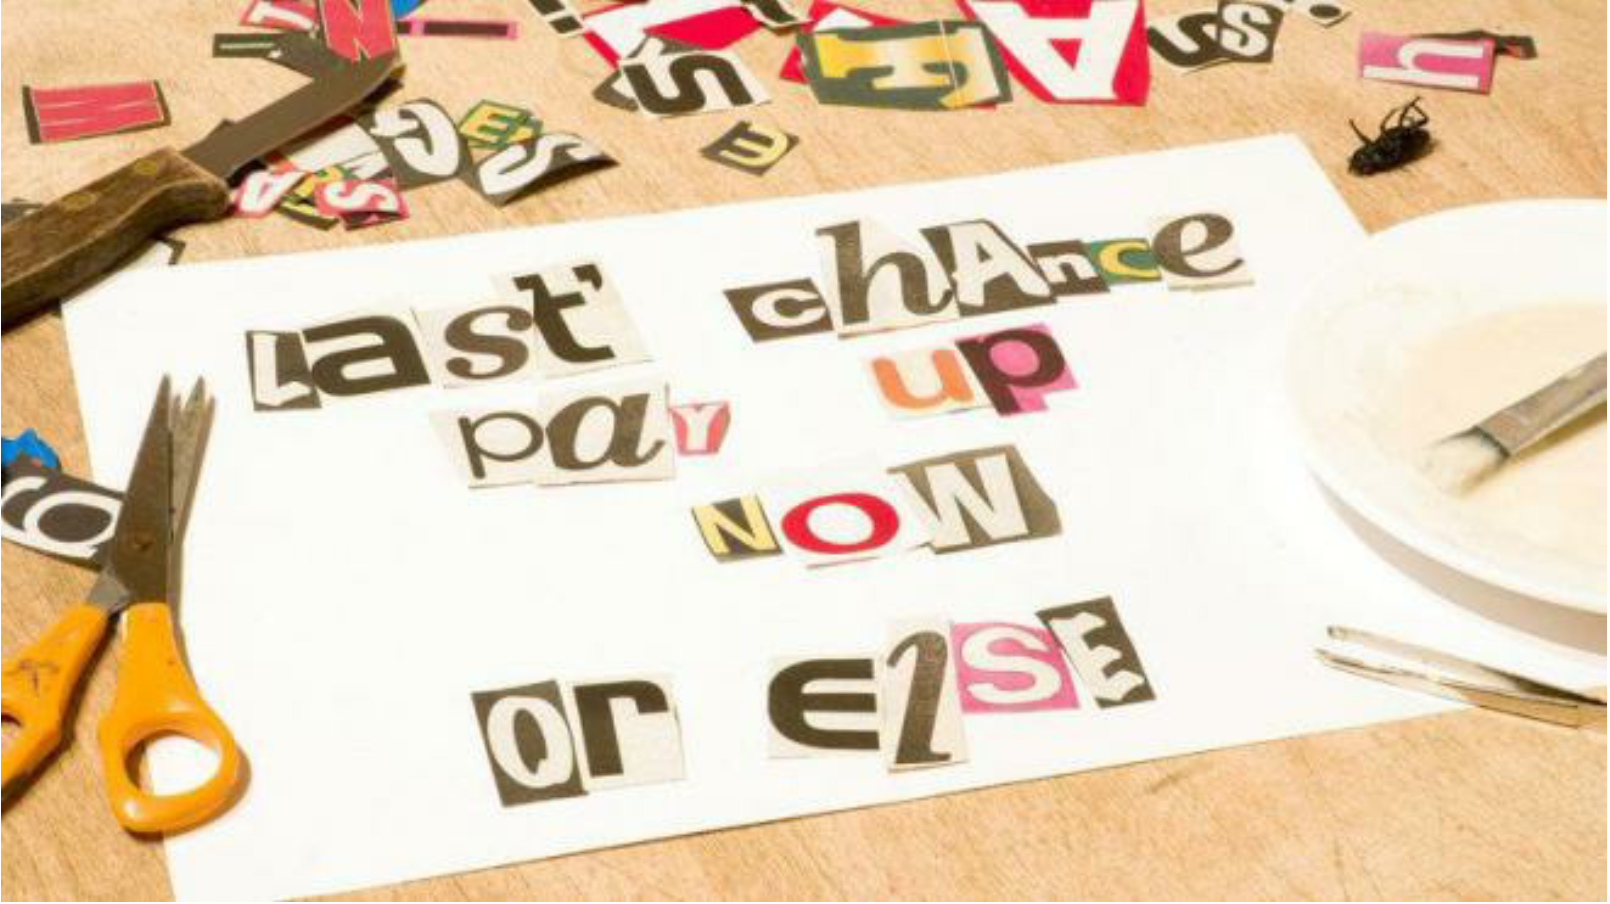
\includegraphics[scale=0.2]{letters.png}
\end{center} 

\newpage 

\subsection*{[10]  Упражнение 4 (Вспомнить все)}

Костя работает в ИПЭИ. Каждый месяц ему на карточку капают бабосики. Костя тратит их на Гиннес в текущем месяце ($C_1$) или может отложить их на следующий месяц ($C_2$). Выбор его потребления зависит от реальной ставки $r$. Однако ЦБ решил, что пора снижать ставку, и Костя, зная свою функцию полезности, хочет нарисовать на графике как изменится его потребление в текущем и будущем месяцах.  

Текущее бюджетное ограничение показано на графике: 

\begin{center}
	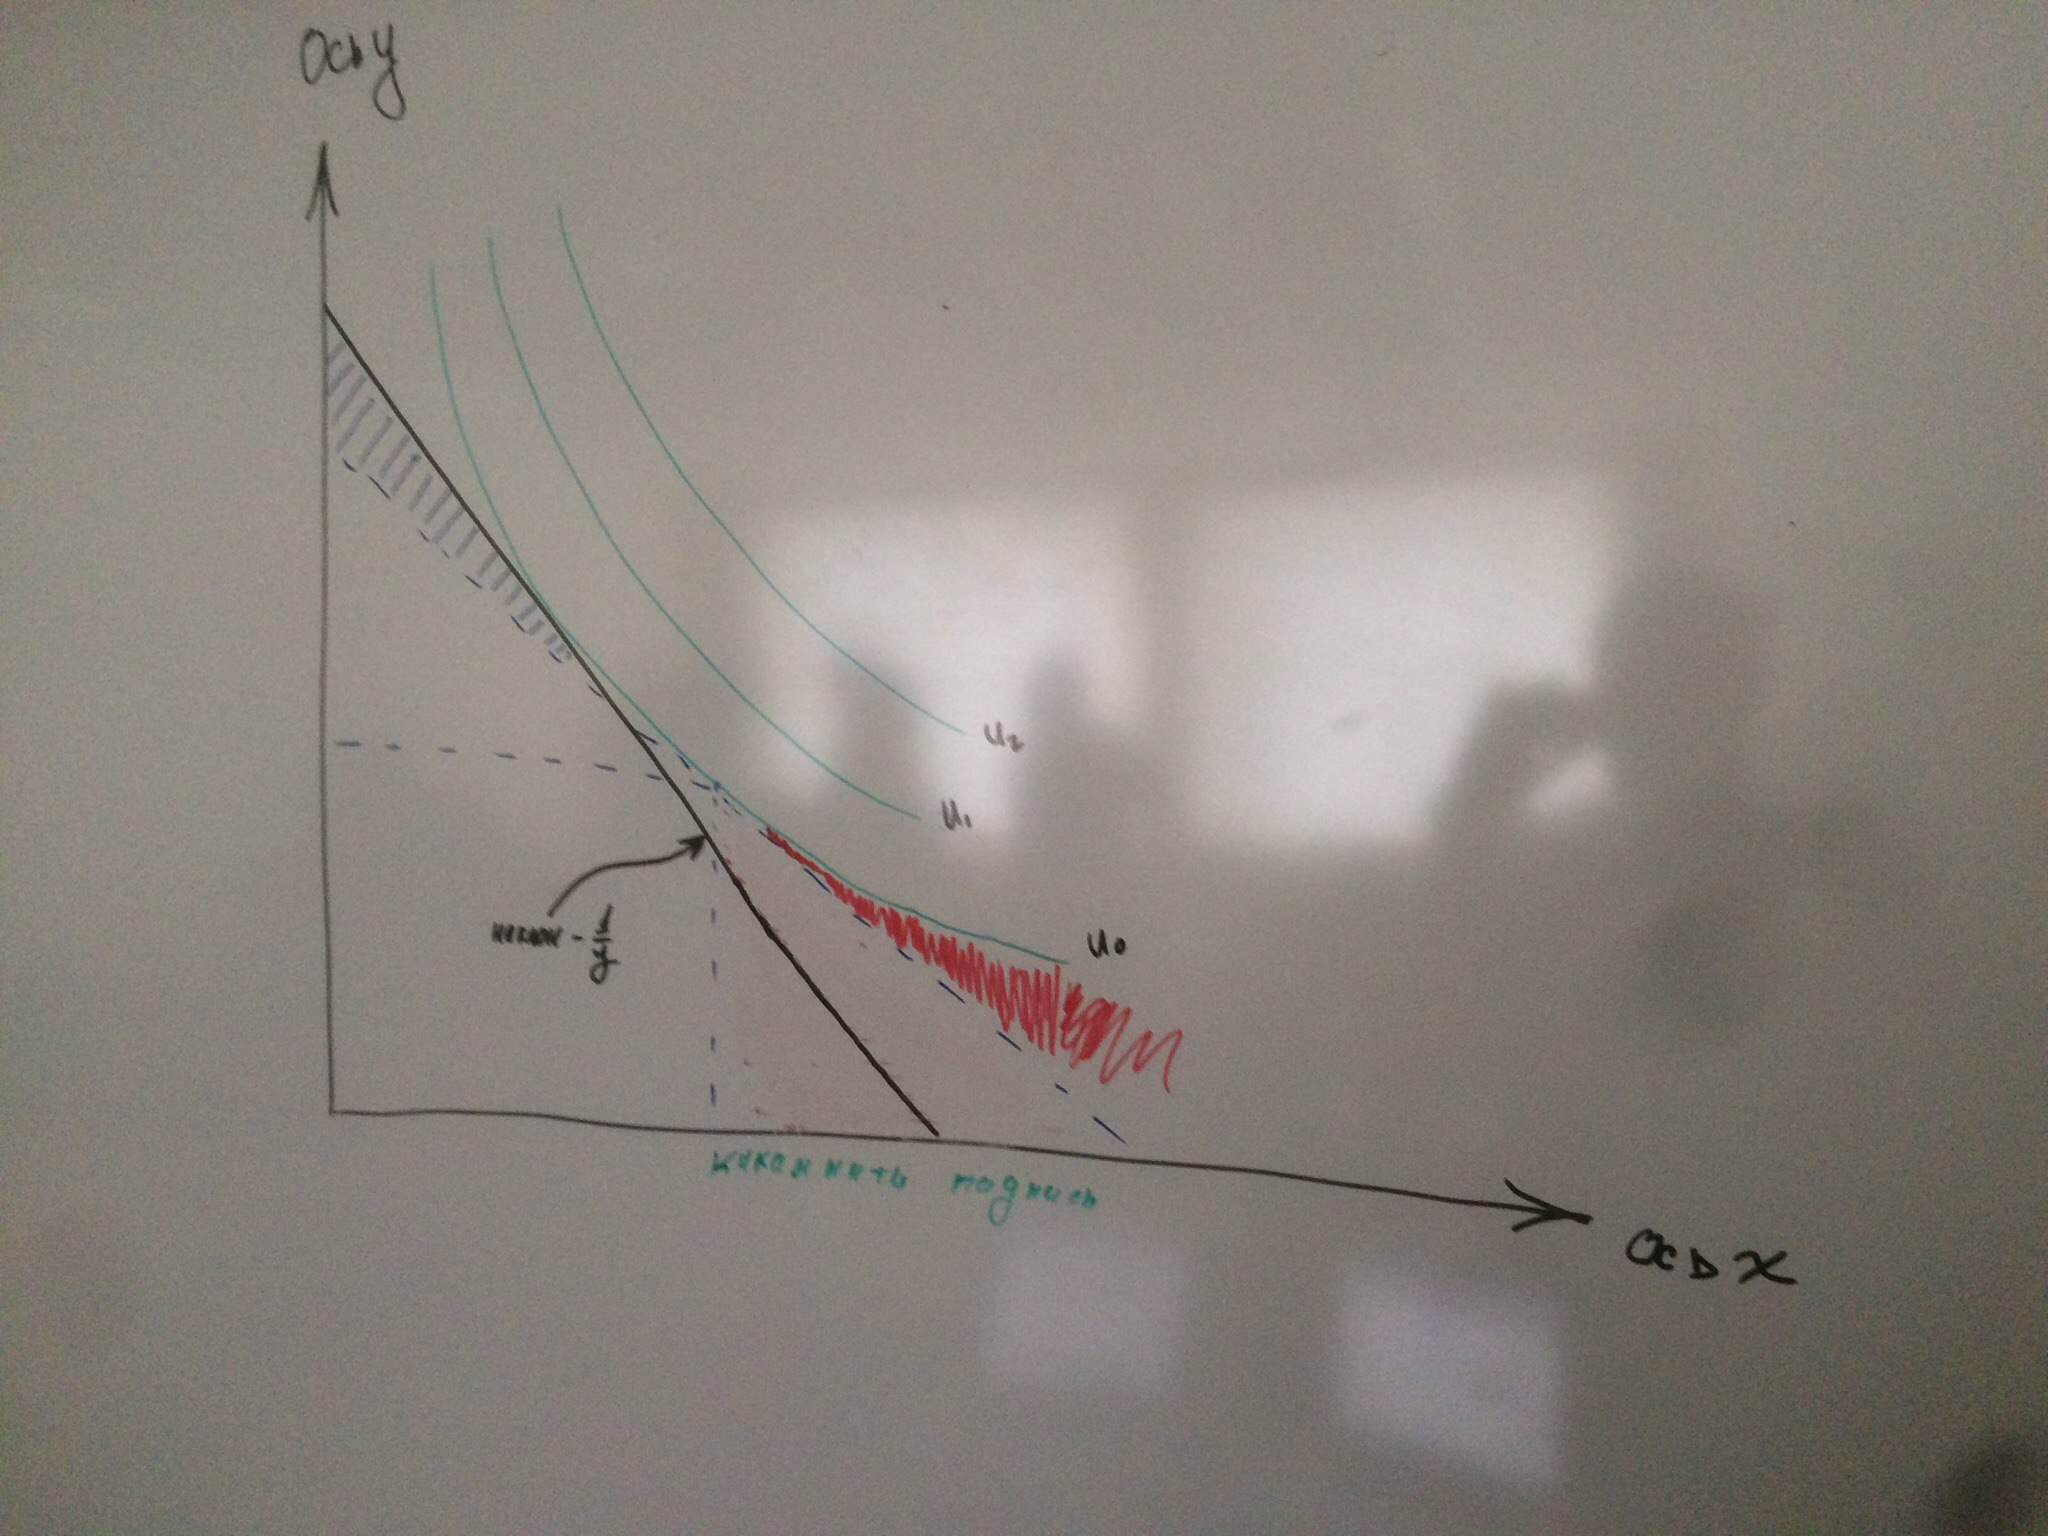
\includegraphics[scale=0.18]{buogr.jpg}
\end{center} 

Такая картинка не нравится Косте. Он хочет перерисовать её в TikZ. 


Ваша задача нарисовать график бюджетного ограничения и показать изначальное равновесие,  равновесие после изменения ставки, причем вам нужно отдельно показать эффект замещения и эффект дохода, показать как изменится потребление каждого из благ (как в результате действия каждого из эффектов, так и суммарно, предположим, что эффект замещения является доминирующим). 

 Мы предполагаем, что предпочтения Кости описываются функцией Кобба-Дугласа с постоянной отдачей от масштаба, а доход Кости в каждом месяце составляет $Y_i$. Дополнительно предположим, что Костя является кредитором.
 
К тому же Костя хочет, чтобы: 

\begin{enumerate}
	
\item  Оси были с подписями, с красивыми изогнутыми остриями стрелок.
\item  Бюджетное ограничение выглядело солидно. Костя же научный сотрудник! 
\item Поворот бюджетного ограничения должен выглядеть менее солидно. Например, пунктирно. 
\item  Кривые безразличия должны затухать, то есть становиться более прозрачными, в сторону увеличения полезности.
\item  Кривые безразличия должны быть подписаны. 
\item  Одну из функций на графике подписать изогнутой стрелочкой. 
\item Две зажатые между бюджетными линиями области должны быть закрашены разной штриховкой. 
\item Для лучшей читаемости графика используйте разные цвета.
\end{enumerate}

\section*{[5]  Бонус (Мы же икономисты)}

Опишите словами, полученный результат, какой экономический смысл несет такая модель? Проинтерпретируйте смысл $r$ в данной модели. 


\end{document}
